\documentclass[10pt,a4paper]{article}
\usepackage{preamble}

\def\FS{Formelsammlung}
\def\Fach{Signale und Systeme}
\title{\FS \ \Fach}
\author{Ayham Alhalaibi}
\date{\today}
\def\MatNr{SECRET} % DONT PUSH TO PUBLIC REMOTE REPO
\def\Semester{Wintersemster 21/22}

\begin{document}

\pagenumbering{gobble}
\begin{titlepage}
\thispagestyle{empty}

\begin{center}
\includegraphics[width=0.7\textwidth]{~/texmf/tex/latex/oth/logos/OTHR_OTHR_Logo.pdf}\\
\vspace*{\stretch{1}}
\Huge
\textsc{\MyTitle}\\
\vspace*{\stretch{0.25}}
\normalsize
\Semester

\vspace*{\stretch{2}}
{\renewcommand{\arraystretch}{1.5}
\begin{tabular}{l l}
    Name:  & \hspace{4cm}\MyAuthor \\
    Matrikelnummer:  & \hspace{4cm}\MatNr\\
    Letzte Änderung:  & \hspace{4cm}\MyDate\\
    Lizenz:  & \hspace{4cm}GPLv3
\end{tabular}
}
\vspace*{\stretch{1}}

\end{center}
\end{titlepage}

\newpage


\tableofcontents\clearpage

% \setlength{\columnsep}{1pt}
\raggedcolumns
\begin{multicols*}{2}
\pagestyle{fancy}
\lhead{\FS\\\Fach}
\rhead{\MyAuthor\\\Semester}
\cfoot{\vspace{-20pt}\thepage}
\pagenumbering{arabic}

\section{Signale im Zeitbereich}
  \subsection{Signalcharakterisierung}
  \begin{enumerate}
      \item{\textbf{Kontinuierlich \hfill $\longleftrightarrow$ \hfill Diskret}}
      \item{\textbf{Deterministisch \hfill $\longleftrightarrow$ \hfill Stochastisch}}\\
          Deterministische Signale sind mathematisch beschreibbar, im gegensatz
          zu stochastischen Signalen die dem Zufall unterworfen sind
      \item{\textbf{Periodisch \hfill $\longleftrightarrow$ \hfill Aperiodisch}}\\
          \begin{mdframed}[style=exercise]
              periodisch wenn, $x(t)=x(t+T_p)$ gilt.

              $T_p$ hei{\ss}t Grundperiode.
          \end{mdframed}
      \item{\textbf{Gerade \hfill $\longleftrightarrow$ \hfill Ungerade:}}\\
          \begin{mdframed}[style=exercise,frametitle=Zerlegung des Signals:]
              - gerader Anteil: \[x_G=\frac{1}{2}\left[x(t)+x(t-1)\right]\]
              - ungerader Anteil: \[x_U=\frac{1}{2}\left[ x(t)-x(-t) \right]\]
          \end{mdframed}
          \begin{center}
              \includegraphics[width=0.43\textwidth]{Signale/gerade_ungerade_signal}
          \end{center}
      \item{\textbf{Energiesignal \hfill $\longleftrightarrow$ \hfill Leistungssignal}}
          \begin{mdframed}[style=exercise]
              Energie: \[E_x=\int_{t=-\infty}^{+\infty}\lvert x(t)\rvert^2 dt\]
              Leistung: \[P_x=\lim_{T\to\infty}\frac{1}{2T}\int_{-T}^{+T}\lvert x(t)\rvert^2 dt\]
          \end{mdframed}
      \item{\textbf{Korrelation}}\\
          Die Korrelationsfunktion ist eine Ma{\ss} f\"ur die \"Ahnlichkeit
          zweier deterministischer Energiesignale.
          \begin{mdframed}[style=exercise,frametitle=Korrelationsfunktion]
              \[
                  r_{xy}(\tau) = \int_{-\infty}^{\infty}x(t)\cdot y(t+\tau)dt
              \]
          \end{mdframed}
      \item{\textbf{Transformation}}\\
          Signale k\"onnenn modifiziert werden durch Ver\"andern der
          unabh\"angigen Variablen:
          \begin{itemize}
              \item Zeitverschiebung
              \item Zeitdehnung und Stauchung
              \item Zeitumkehr
          \end{itemize}
          \begin{mdframed}[style=exercise]
              \[
                  x_2(t) = x_1(-at+b)
              \]
          das Argument von $x_1(\tau)$ stellt eine Abbildung $t\rightarrow\tau$
          dar, daher bewirkt
          \begin{itemize}
              \item{$+b / -b\ (b > 0)$ eine Verschiebung von $x_1(\tau)$ nach links / rechts}

              \item{eine Multiplikation mit a / Division durch a $(a>1)$ eine Stauchung /
                  Streckung von $x_1(\tau)$}

              \item{Multiplikation mit -1 eine Spiegelung an der Ordinatenachse}
          \end{itemize}
          Die Reihenfolge der Schritte ist nicht \textbf{EGAL}:\\
          \color{red}{erst Verschieben um $b$, dann Skalieren/Invertieren mit $-a$}
          \end{mdframed}
  \end{enumerate}
  \subsection{Elementarsignale}
  \begin{mdframed}[style=exercise]
      \begin{itemize}
          \item{Sprungfunktion $\varepsilon$}
          \[ \varepsilon(t) =
             \begin{cases}
                 0 & \text{f\"ur } t < 0\\
                 1 & \text{f\"ur } t \geq 0
             \end{cases}
          \]
          \item{Dirac $\delta$}
          \[
              \int_{t=-\infty}^{\infty} \delta(t)dt = 1
          \]
          Eigenschaften:
          \begin{itemize}
              \item{H\"ohe unendlich}
              \item{Fl\"ache = 1}
              \item{Zusammenhang mit Sprungfunktion}\\
                  $\int_{\tau=-\infty}^{t}\delta(\tau)d\tau =
                  \varepsilon(t)$ bzw.  $\dfrac{d}{dt}\varepsilon(t) =
                  \delta(t)$
              \item{Ausblendeigenschaft}
                  \[
                      \delta(t-t_0)\cdot y(t) = \delta(t-t_0)\cdot y(t_0)
                  \]
              \item{Zeitskalierung: }
                  $\delta(at)=\frac{1}{\lvert a\rvert}\delta(t)$
          \end{itemize}
          \item{Dreieckimpuls $\Lambda$}
          \[ \Lambda(t) =
             \begin{cases}
                 0 & \text{f\"ur } \vert t\rvert > 1\\
                 1 & \text{f\"ur } \vert t\rvert \leq 1
             \end{cases}
          \]
          \item{Rechteckfunktion $rect$}
          \[ rect(t) =
             \begin{cases}
                 1 & \text{f\"ur } \vert t\rvert \leq \frac{1}{2}\\
                 0 & \text{f\"ur } \vert t\rvert > \frac{1}{2}
             \end{cases}
          \]
          Darstellbar durch:\\ $rect(t) = \varepsilon\cdot\left( t+\frac{1}{2} \right)-\varepsilon\cdot\left( t-\frac{1}{2} \right)$
          \item{Komplexe Exponentialfunktion}
          \[ \Lambda(t) =
             \begin{cases}
                 0 & \text{f\"ur } \vert t\rvert > 1\\
                 1 & \text{f\"ur } \vert t\rvert \leq 1
             \end{cases}
          \]
      \end{itemize}
  \end{mdframed}

\section{Systeme}
\subsection{Eigenschaften}
\begin{enumerate}
  \item{\textbf{Speicher}}\\
      % \begin{mdframed}[style=exercise]
          \bulletpt Frei: wird durch eine xy-Kennlinie vollständig
          beschrieben
          \[
              \text{z.B. \ }y(t)=\frac{R_1}{R_1+R_2}\cdot x(t)
          \]
          \bulletpt behaftet: Bei diesen Systemen ist keine
          vollständige Beschreibung durch eine xy-Kennline möglich
          \[
              \text{z.B. \ }y(t) = x(t)+2x(t-1)
          \]
      % \end{mdframed}
  \item{\textbf{Kausalit\"at}}\\
      % \begin{mdframed}[style=exercise]
           Ausgangssignal hängt nur vom aktuellen und vorherigen
           Eingangssignal ab
          \[
              \text{Kausal: z.B. \ }y(t) =
              \int\displaylimits_{t-5}^{t}x(\tau)d\tau
          \]
          \[
              \text{Akausal: z.B. \ }y(t) = x(t+1)-x(t-1)
          \]
      % \end{mdframed}

      \underline{Speicherfreiheit \& Kausalit\"at:} Aus Speicherfreiheit
      folgt Kausalität, aber nicht umgekehrt.
  \item{\textbf{Stabilit\"at}}\\
  (Bounded Input $\rightarrow$ Bounded Output)\\BIBO Stabilit\"at:
  kleines/beschr\"anktes Eingangssignal $\rightarrow$ kleine/beschr\"ankte
  Antwort.\\
  \includegraphics[width=.9\columnwidth]{Systeme/BIBO_anschaulich}\\
  % \begin{mdframed}[style=exercise]
      z.B. f\"ur stabiles System
  \[
      y(t) = 50\cdot x^3(t)
  \]\\
      z.B. f\"ur instabiles System
  \[
      y(t) = e^{t}\cdot x(t)
  \]
  % \end{mdframed}
  \item{\textbf{Zeitinvariant$\leftrightarrow$Zeitvariant}}\\
  \bulletpt invariant: Systeme \"andern sich \textbf{nicht} bei einer
  Zeitverschiebung.\\
  \bulletpt variant: Verschobenes Eingangssignal $\rightarrow$
  verschobenes Ausgangssignal
  \item{\textbf{Liniarit\"at}}\\
      Ein System ist linear, wenn das Superpositionsprinzip gilt:
      Linearkombination von Eingangssignalen ruft entsprechende
      Linearkombination der Ausgangssignale hervor
      \begin{mdframed}[style=exercise,frametitle=Bedeutung Liniarit\"at]
          eine Verdopplung der Eingangsgröße (z.B. Spannung) führt auch zu
          einer Verdopplung der Ausgangsgröße.
      \end{mdframed}
\end{enumerate}
\subsection{LTI-Systeme (Linear time-invariant Systems)}
\subsubsection{Ein-/Ausgangsbeziehung}
\begin{itemize}
  \item Addition
  \item Multiplikation
  \item Differentiation
  \item Integration
  \item Zeitverschiebung(Verz\"ogerung)
\end{itemize}
\subsubsection{Faltung}
Aus der Impulsantwort eines LTI-Systems und dem Eingangssignal lässt sich das
Ausgangssignal durch Faltung bestimmen:
\begin{mdframed}[style=exercise]
  \[
      y(t)=x(t)*h(t) \rightarrow (*)\text{ Faltung Operator}
  \]
  \[
      \boxed{y(t) = \int_{-\infty}^{+\infty} x(\tau)\cdot h(t-\tau)d\tau}
  \]
  \bulletpt Der Dirac-Impuls ist das neutrale Element der Faltung
  \[
      x(t)*\delta(t)=x(t)
  \]
  \bulletpt Eine Faltung mit einem verschobenen Dirac-Impuls führt zur Verschiebung
  des Signals:
  \[
      x(t)* \delta(t - a) = x(t - a)
  \]
\end{mdframed}
\begin{mdframed}[style=exercise,frametitle=Rechenregeln]
  \begin{itemize}
      \item{$x_1(t)*x_2(t)=x_2(t)*x_1(t)$}
      \item{$x_1(t)*[x_2(t)*x_3(t)]=[x_1(t)*x_2(t)]*x_3(t)$}
      \item{$x_1(t)*[x_2(t)+x_3(t)]=x_1(t)*x_2(t)+x_1(t)*x_3(t)$}
  \end{itemize}
\end{mdframed}
\subsection{Frequenzgang \& \"Ubertragungsfunktion}
\begin{mdframed}[style=exercise]
  \begin{itemize}
      \item{\textbf{Frequenzgang}}\\
          \[
              \underline{H}(\omega) =
              \frac{\underline{Y}(\omega)}{\underline{X}(\omega)} =
              \frac{\underline{U_2}(\omega)}{\underline{U_1}(\omega)}
          \]
      \item{\textbf{Amplitudengang}}\\
          \[
              A(\omega) = |\underline{H}(\omega)| =
              \frac{|\underline{Y}(\omega)|}{|\underline{X}(\omega)|}
              \begin{cases}
                  > 1 & \text{Verst\"arkung}\\
                  < 1 & \text{D\"ampfung}
              \end{cases}
          \]
      \item{\textbf{Phasengang}}\\
          \[
              \varphi_H(\omega) = \text{arg}\{\underline{H}(\omega)\} =
              \varphi_Y(\omega) - \varphi_X(\omega)
          \]
          \[
              \varphi_H = \text{arctan}(\frac{\mathfrak{Im}}{\mathfrak{Re}})
          \]
      \item{\textbf{Eigenfunktion}}\\
          \[
              y(t) = \lambda\cdot x(t)
              \begin{cases}
                  x(t): & \text{Eigenfunktion}\\
                  \lambda: & \text{Eigenwert}(\lambda\in\mathbb{C})
              \end{cases}
          \]
  \end{itemize}
\end{mdframed}
\begin{mdframed}[style=exercise]
  jede komplexe Exponentialfunktion $x(t) = \e^{st}$ ist Eigenfunktion
  jedes beliebigen LTI-Systems $S$:
  \[
      y(t) = S\left\{ \e^{st} \right\} = \lambda\cdot \e^{st}
  \]
  Eigenwert kann wie folgt berechnet werden:
  \[
      \lambda = \underline{H}(s) = \int_{-\infty}^{+\infty} h(\tau)\  \e^{-st} d\tau
  \]
  \begin{itemize}
      \item{\textbf{Erweiterung der komplexen Wechselstromrechnung}}\\
          Die harmonische Exponentialfunktion $e^{j\omega t}$ ist ein
          sonderfall von $e^{st}$ mit $s=j\omega$
          \[
              \sigma \triangleq Amplitude
              \begin{cases}
                  \sigma \leq 0 & \text{exponentiell abklingend}\\
                  \sigma = 0 & \text{konstante Amplitude}\\
                  \sigma \geq 0 & \text{exponentiell zunehmend}
              \end{cases}
          \]
          \[
              \omega \triangleq Rotation
              \begin{cases}
                  \omega \leq 0 & \text{Zeiger rotiert mit UZS}\\
                  \omega = 0 & \text{Zeiger rotiert nicht}\\
                  \omega \geq 0 & \text{Zeiger rotiert gegen UZS}
              \end{cases}
          \]
  \end{itemize}
\end{mdframed}
% \[
%   \boxed{
%   \begin{circuitikz}[scale=1,transform shape]
%       \draw(0,0) to[generic] node[anchor=east,yshift=-20pt]{$\underline{Z}(s)\mathrm{=}R$} (2,0);
%       \draw(3,0) to[L] node[anchor=east,yshift=-20pt, xshift=5pt]{$\underline{Z}(s)\mathrm{=}s\cdot L$} (5,0);
%       \draw(6,0) to[C, l=] node[anchor=east, yshift=-20pt, xshift=6pt]{$\underline{Z}(s)\mathrm{=}\frac{1}{s\cdot C}$} (8,0);
%   \end{circuitikz}
%   }
% \]

\begin{mdframed}[style=exercise,frametitle=Komplexe \"Ubertragungsfunktion]
  \footnotesize
  \[
      \underline{H}(s)=\frac{\underline{Y}(s)}{\underline{X}(s)}=\frac{\underline{U_2}(s)}{\underline{U_1}(s)}=\frac{\text{komplexer
      Zeiger des Ausgangssignals}}{\text{komplexer Zeiger des
      Eingangssignals}}
  \]
  \normalsize
  Die Übertragungsfunktion hängt von der komplexen\linebreak Frequenz
  $s=\sigma+j\omega$ ab.
\end{mdframed}

\subsubsection{Pegel}
    \begin{mdframed}[style=exercise]
        Energiegröße: $\quad a = 10\cdot \lg\dfrac{P_1}{P_2}dB $\\
        Feldgröße: $\qquad a = 20\cdot \lg\dfrac{U_1}{U_2}dB $
    \end{mdframed}

\subsection{Pole und Nullstellen}
\[
    H(s)=\frac{\sum_{m=0}^{M} b_{m} \cdot s^{m}}{\sum_{n=0}^{N} a_{n} \cdot s^{n}}
\]
Die Koeffizienten an und bm ergeben sich aus den Bauelementen und sind reell.
\begin{mdframed}[style=exercise]
    \begin{align*}
        \underline{H}(s) &= \frac{\textsc{Summe aller Nullstellen}}{\textsc{Summe aller Pole}}\\
        &=\frac{b_{M}}{a_{N}} \cdot \frac{\left(s-s_{o 1}\right) \cdot\left(s-s_{o
        2}\right) \cdot \ldots \cdot\left(s-s_{o M}\right)}{\left(s-s_{x 1}\right)
        \cdot\left(s-s_{x 2}\right) \cdot \ldots \cdot\left(s-s_{x N}\right)}
    \end{align*}
    $k=\dfrac{b_M}{a_N}$ ist der Maßstabfaktor
\end{mdframed}
\textbf{Bei stabilen Systemen müssen alle Pole in der linken komplexen Halbebene liegen.}

\subsection{Elementare Übertragungsglieder}
\footnotesize
    P-Glied , D-Glied , I-Glied , PT1-Glied
\normalsize
Für mehr sehe externe Tabelle.

\subsection{Zusammenschalten von Übertragungsgliedern}
\begin{mdframed}[style=exercise]
\begin{itemize}
    \item Kettenschaltung\\
        \textbf{Multiplikation} der Einzelübertragungsfunktionen.
        \[
            \boxed{\underline{H}_{e}(s)=\underline{H}_{B}(s) \cdot \underline{H}_{A}(s)=\underline{H}_{A}(s) \cdot \underline{H}_{B}(s)}
        \]
        \begin{center}
            \includegraphics[width=0.7\columnwidth]{Kettenschaltung_Uebertragungsglieder}
            \[
                \underline{Y}_{B}=\underline{H}_{B}(s) \cdot \underline{X}_{B}=\underline{H}_{B}(s) \cdot \underline{Y}_{A}=\underline{H}_{B}(s) \cdot \underline{H}_{A}(s) \cdot \underline{X}_{A}
            \]
        \end{center}
        Rückwirkungsfreiheit gewährleistet sein.
    \item Parallelschaltung\\
        \textbf{Summe} der Einzelübertragungsfunktionen.
        \[
            \boxed{\underline{H}_{e}(s)=\underline{H}_{B}(s) + \underline{H}_{A}(s)}
        \]
        \begin{center}
            \includegraphics[width=0.6\columnwidth]{Parallel_Uebertragungsglieder}
            \begin{align*}
                \underline{Y}&=\underline{Y}_{A} \pm \underline{Y}_{B}\\
                             &=\underline{H}_{A}(s) \cdot \underline{X}_{A} \pm \underline{H}_{B}(s) \cdot \underline{X}_{B}\\
                             &=\left(\underline{H}_{A}(s)+\underline{H}_{B}(s)\right) \cdot \underline{X}
            \end{align*}
        \end{center}
    \item Rückkopplung
        \[
            \boxed{\underline{H}_{e}(s)=\frac{\underline{H}_{A}(s)}{1\pm\underline{H}_{A}(s) \cdot \underline{H}_{B}(s)}}
        \]
        \begin{center}
            \includegraphics[width=0.6\columnwidth]{Rueckkopplung_Uebertragungsglieder}\\
            Mitkopplung: $y_A$ vergrößert $x_A$\\
            Gegenkopplung $y_A$ verkleinert $x_A$
        \end{center}

\end{itemize}
\end{mdframed}

\subsection{Bode Diagramm}
\begin{itemize}
    \item Bode Diagramm von Kettenschaltung\\
        Ergibt sich durch \textbf{Addition der Bodediagramme} der einzelnen Glieder.
    \item Bode Diagramm der inversen Übertragungsfunktion\\
        Ergibt sich durch \textbf{Spiegelung an der X-Achse}.
\end{itemize}

\clearpage
\section{Zweitore - Vierpoltheorie}
\subsection{Zweitorgleichungen}
% \includegraphics[width=\columnwidth]{Zweipole/Zweitorgleichungen}
\begin{mdframed}[style=exercise]
    \begin{itemize}
        \item{Admittanzform/ Admittanzmatrix \textbf{Y}:}
        \begin{align*}
            \begin{split}
                \underline{I}_1 &= \underline{Y}_{11}\cdot\underline{U}_1 + \underline{Y}_{12}\cdot\underline{U}_2\\
                \underline{I}_2 &= \underline{Y}_{21}\cdot\underline{U}_1 + \underline{Y}_{22}\cdot\underline{U}_2
            \end{split}
        \left\} \
            \begin{pmatrix}
                \underline{I}_1 \\
                \underline{I}_2
            \end{pmatrix} = \textbf{\underline{Y}}\cdot
            \begin{pmatrix}
                \underline{U}_1 \\
                \underline{U}_2
            \end{pmatrix}
        \right.
        \end{align*}
        \item{Impedanzform/ Impedanzmatrix \textbf{Z}:}
            \begin{align*}
                \begin{split}
                \underline{U}_1 &=\underline{Z}_{11}\cdot\underline{I}_1 + \underline{Z}_{12}\cdot\underline{I}_2 \\
                \underline{U_2} &=\underline{Z}_{21}\cdot\underline{I}_1 + \underline{Z}_{22}\cdot\underline{I}_2
                \end{split}
            \left\} \
                \begin{pmatrix}
                    \underline{U}_1 \\
                    \underline{U}_2
                \end{pmatrix} = \textbf{\underline{Z}}\cdot
                \begin{pmatrix}
                    \underline{I}_1 \\
                    \underline{I}_2
                \end{pmatrix}
            \right.
            \end{align*}
        \item{Hybridform 1/ Reihenparallelmatrix \textbf{H}:}
            \begin{align*}
                \begin{split}
                    \underline{U}_1 &= \underline{H}_{11}\cdot\underline{I}_1 + \underline{H}_{12}\cdot\underline{U}_2 \\
                    \underline{I}_2 &= \underline{H}_{21}\cdot\underline{I}_1 + \underline{H}_{22}\cdot\underline{U}_2
                \end{split}
            \left\} \
                \begin{pmatrix}
                    \underline{U}_1 \\
                    \underline{I}_2
                \end{pmatrix} = \textbf{\underline{H}}\cdot
                \begin{pmatrix}
                    \underline{I}_1 \\
                    \underline{U}_2
                \end{pmatrix}
            \right.
            \end{align*}
            \item{Hybridform 2/ Parallelreihenmatrix \textbf{C}:}
            \begin{align*}
                \begin{split}
                    \underline{I}_1 &= \underline{C}_{11}\cdot\underline{U}_1 + \underline{C}_{12}\cdot\underline{I}_2 \\
                    \underline{U}_2 &= \underline{C}_{21}\cdot\underline{U}_1 + \underline{C}_{22}\cdot\underline{I}_2
                \end{split}
            \left\} \
                \begin{pmatrix}
                    \underline{I}_1 \\
                    \underline{U}_2
                \end{pmatrix} = \textbf{\underline{C}}\cdot
                \begin{pmatrix}
                    \underline{U}_1 \\
                    \underline{I}_2
                \end{pmatrix}
            \right.
            \end{align*}
            \item{Kettenform/ Kettenmatrix \textbf{A}:}
                \begin{align*}
                    \begin{split}
                        \underline{U}_1 &= \underline{A}_{11}\cdot\underline{U}_2 + \underline{A}_{12}\cdot-\underline{I}_2 \\
                        \underline{I}_1 &= \underline{A}_{21}\cdot\underline{U}_2 + \underline{A}_{22}\cdot-\underline{I}_2
                    \end{split}
                \left\} \
                    \begin{pmatrix}
                        \underline{U}_1 \\
                        \underline{I}_2
                    \end{pmatrix} = \textbf{\underline{A}}\cdot
                    \begin{pmatrix}
                        \underline{U}_2 \\
                        -\underline{I}_2
                    \end{pmatrix}
                \right.
                \end{align*}
                \item{Kettenform rückwärts/ Kettenmatrix \textbf{B}:}
                    \begin{align*}
                        \begin{split}
                            \underline{U}_2 &= \underline{B}_{11}\cdot\underline{U}_1 + \underline{B}_{12}\cdot-\underline{I}_1\\
                            \underline{I}_2 &= \underline{B}_{21}\cdot\underline{U}_1 + \underline{B}_{22}\cdot-\underline{I}_1
                        \end{split}
                    \left\} \
                    \begin{pmatrix}
                        \underline{U}_2\\
                        \underline{I}_2
                    \end{pmatrix} = \textbf{\underline{B}}\cdot
                    \begin{pmatrix}
                        \underline{U}_1 \\
                        -\underline{I}_1
                    \end{pmatrix}
                \right.
                    \end{align*}
    \end{itemize}
\end{mdframed}

\subsubsection{Parameterumrechnung}
\begingroup
\arraycolsep=1.0pt\def\arraystretch{2.0}
\begin{align*}
    Z && \hspace{0.5cm} Y && \hspace{0.5cm} H && \hspace{0.5cm} A
\end{align*}
\[
    Z\
    \begin{bmatrix}
        \underline{Z}_{11} & \underline{Z}_{12}\\
        \underline{Z}_{21} & \underline{Z}_{22}
    \end{bmatrix}
    \begin{bmatrix}
        \dfrac{\underline{Y}_{22}}{\operatorname{det}\underline{\boldsymbol{Y}}} & \dfrac{-\underline{Y}_{12}}{\operatorname{det} \underline{\boldsymbol{Y}}}\\
        \dfrac{-\underline{Y}_{21}}{\operatorname{det} \underline{\boldsymbol{Y}}} & \dfrac{\underline{{Y}}_{11}}{\operatorname{det} \underline{\boldsymbol{Y}}} \\
    \end{bmatrix}
    \begin{bmatrix}
        \dfrac{\operatorname{det}\underline{\boldsymbol{{H}}}}{\underline{H}_{22}} & \dfrac{\underline{H}_{12}}{\underline{H}_{22}} \\
        \dfrac{-\underline{H}_{21}}{\underline{H}_{22}} & \dfrac{1}{\underline{H}_{22}}
    \end{bmatrix}
    \begin{bmatrix}
        \dfrac{\underline{A}_{11}}{\underline{A}_{21}} & \dfrac{\operatorname{det}\underline{\boldsymbol{A}}}{\underline{A}_{21}}\\
        \dfrac{1}{\underline{A}_{21}} & \dfrac{\underline{{A}}_{22}}{\underline{A}_{21}} \\
    \end{bmatrix}
\]
\[
    Y\
    \begin{bmatrix}
        \dfrac{\underline{Z}_{22}}{\operatorname{det}\underline{\boldsymbol{Z}}} & \dfrac{-\underline{Z}_{12}}{\operatorname{det} \underline{\boldsymbol{Z}}}\\
        \dfrac{-\underline{Z}_{21}}{\operatorname{det} \underline{\boldsymbol{Z}}} & \dfrac{\underline{{Z}}_{11}}{\operatorname{det} \underline{\boldsymbol{Z}}} \\
    \end{bmatrix}
    \begin{bmatrix}
        \underline{Y}_{11} & \underline{Y}_{12}\\
        \underline{Y}_{21} & \underline{Y}_{22}
    \end{bmatrix}
    \begin{bmatrix}
        \dfrac{1}{\underline{H}_{11}} & \dfrac{-\underline{H}_{12}}{\underline{H}_{11}} \\
        \dfrac{\underline{H}_{21}}{\underline{H}_{11}} & \dfrac{\operatorname{det}\underline{\boldsymbol{{H}}}}{\underline{H}_{11}}
    \end{bmatrix}
    \begin{bmatrix}
        \dfrac{\underline{A}_{22}}{\underline{A}_{12}} & \dfrac{-\operatorname{det}\underline{\boldsymbol{A}}}{\underline{A}_{12}}\\
        \dfrac{-1}{\underline{A}_{12}} & \dfrac{\underline{{A}}_{11}}{\underline{A}_{12}} \\
    \end{bmatrix}
\]
\[
    H\
    \begin{bmatrix}
        \dfrac{\operatorname{det}\underline{\boldsymbol{{Z}}}}{\underline{Z}_{22}} & \dfrac{\underline{Z}_{12}}{\underline{Z}_{22}} \\
        \dfrac{-\underline{Z}_{21}}{\underline{Z}_{22}} & \dfrac{1}{\underline{Z}_{22}}
    \end{bmatrix}
    \begin{bmatrix}
        \dfrac{1}{\underline{Y}_{11}} & \dfrac{-\underline{Y}_{12}}{\underline{Y}_{11}} \\
        \dfrac{\underline{Y}_{21}}{\underline{Y}_{11}} & \dfrac{\operatorname{det}\underline{\boldsymbol{{Y}}}}{\underline{Y}_{11}}
    \end{bmatrix}
    \begin{bmatrix}
        \underline{H}_{11} & \underline{H}_{12}\\
        \underline{H}_{21} & \underline{H}_{22}
    \end{bmatrix}
    \begin{bmatrix}
        \dfrac{\underline{A}_{12}}{\underline{A}_{22}} & \dfrac{\operatorname{det}\underline{\boldsymbol{A}}}{\underline{A}_{22}}\\
        \dfrac{-1}{\underline{A}_{22}} & \dfrac{\underline{{A}}_{21}}{\underline{A}_{22}} \\
    \end{bmatrix}
\]
\[
    A\
    \begin{bmatrix}
        \dfrac{\underline{Z}_{11}}{\underline{Z}_{21}} & \dfrac{\operatorname{det}\underline{\boldsymbol{Z}}}{\underline{Z}_{21}}\\
        \dfrac{1}{\underline{Z}_{21}} & \dfrac{\underline{{Z}}_{22}}{\underline{Z}_{21}} \\
    \end{bmatrix}
    \begin{bmatrix}
        \dfrac{-\underline{Y}_{22}}{\underline{Y}_{21}} & \dfrac{-1}{\underline{Y}_{21}}\\
        \dfrac{-\operatorname{det}\underline{\boldsymbol{Y}}}{\underline{Y}_{21}} & \dfrac{-\underline{{Y}}_{11}}{\underline{Y}_{21}} \\
    \end{bmatrix}
    \begin{bmatrix}
        \dfrac{-\operatorname{det}\underline{\boldsymbol{{H}}}}{\underline{H}_{21}} & \dfrac{-\underline{H}_{11}}{\underline{H}_{21}} \\
        \dfrac{-\underline{H}_{22}}{\underline{H}_{21}} & \dfrac{-1}{\underline{H}_{21}}
    \end{bmatrix}
    \begin{bmatrix}
        \underline{A}_{11} & \underline{A}_{12}\\
        \underline{A}_{21} & \underline{A}_{22}
    \end{bmatrix}
\]
\endgroup

% \includegraphics[width=\columnwidth,height=9cm]{Zweipole/Parameterumrechnung}\\

\subsection{Zusammenschalten von Zweitoren}

\begin{mdframed}[style=exercise]
\begin{itemize}
    \item Reihenschaltung:
        \begin{center}
            \includegraphics[width=0.5\textwidth]{Zweipole/Reihenschaltung_Zweitore}
        \[
            \left[ \underline{Z} \right] = \left[ \underline{Z}_1 \right] + \left[ \underline{Z}_2 \right]
        \]
        \end{center}
    \item Parallelschaltung:
        \begin{center}
            \includegraphics[width=0.6\textwidth]{Zweipole/Parallelschaltung_Zweitoren}
        \[
            \left[ \underline{Y} \right] = \left[ \underline{Y}_1 \right] + \left[ \underline{Y}_2 \right]
        \]
        \end{center}
    \item Kettenschaltung:
        \begin{center}
            \includegraphics[width=0.7\textwidth]{Zweipole/Kettenschaltung_Zweitoren}
        \[
            \left[ \underline{A} \right] = \left[ \underline{A}_1 \right] \cdot \left[ \underline{A}_2 \right]
        \]
        \end{center}
        \footnotesize
        \textsc{Beachte:}\\
        \normalsize Im Allgemeinen gilt $\rightarrow
        \left[ \underline{A}_1 \right] \cdot \left[
        \underline{A}_2 \right] \neq \left[ \underline{A}_2
        \right] \cdot \left[ \underline{A}_1 \right]$
    \item Reihen-Parallelschaltung:
        \begin{center}
            \includegraphics[width=0.5\textwidth]{Zweipole/Reihen-Parallelschaltung_Zweitoren}
        \[
            \left[ \underline{H} \right] = \left[ \underline{H}_1 \right] \cdot \left[ \underline{H}_2 \right]
        \]
        \end{center}
    \item Parallel-Reihenschaltung:
        \begin{center}
            \includegraphics[width=0.5\textwidth]{Zweipole/Parallel-Reihenschaltung_Zweitoren}
        \[
            \left[ \underline{C} \right] = \left[ \underline{C}_1 \right] \cdot \left[ \underline{C}_2 \right]
        \]
        \end{center}
\end{itemize}
\end{mdframed}


\clearpage
\begin{samepage}
    \subsection{Matrizen elementarer Zweitore}
    \begin{center}
        \includegraphics[width=\textwidth]{Zweipole/Matrizen_elementarer_zweitore}\\
        \includegraphics[width=\textwidth]{Zweipole/Matrizen_elementarer_zweitore_1}
    \end{center}
\end{samepage}
\clearpage

\subsubsection{Trennverst\"arker}
\begin{mdframed}[style=exercise]
Ersatzschaltbild eines idealen Trennverst\"arkers:
    \begin{center}
        \includegraphics[width=0.7\textwidth]{Zweipole/Trennverstaerker_esb}
    \end{center}
    \[
        A = \begin{pmatrix}
            \dfrac{1}{v_U} & 0 \\
                  0        & 0
        \end{pmatrix}
    \]
    \[
        \underline{A}_e = \begin{pmatrix}
            \underline{A}_{11} & \underline{A}_{12}\\
            \underline{A}_{21} & \underline{A}_{22}
        \end{pmatrix}
        \cdot
        \begin{pmatrix}
            \dfrac{1}{v_U} & 0 \\
                  0        & 0
        \end{pmatrix}
        = \begin{pmatrix}
            \dfrac{\underline{A}_{11}}{v_U} & 0\\
            \dfrac{\underline{A}_{21}}{v_U} & 0
        \end{pmatrix}
    \]
\end{mdframed}

\subsubsection{Torbedingungen}
Die Torbedingungen werden durch:
    \begin{itemize}
        \item idealen \"Ubertrager
        \item Kurzschlussschleife
        \item Parallelschaltung längssymmetrischer Zweitore
    \end{itemize} erf\"ullt.


für die das Zusammenschalten von Zweitoren müssen diese Bedingungen
eingehalten werden.

\subsection{Zweitor Eigenschaften:}
\begin{itemize}
        % \setlength{\itemindent}{-1em}
    \item Reziprozit\"at (Umkehrbarkeit)
        \begin{center}
            \begin{tabular}{|c|c|}
                \hline
                $Z$&  $Z_{12} = Z_{21}$\\
                \hline
                $Y$&  $Y_{12} = Y_{21}$\\
                \hline
                $A$&  $\operatorname{det}[A] = 1$\\
                \hline
                $H$&  $H_{12} = -H_{21}$\\
                \hline
            \end{tabular}
        \end{center}
        Ein umkehrbares (reziprokes) Zweitor wird\\ nur durch drei Parameter
        beschrieben:

        \footnotesize
        \textbf{(RLCM-Zweitor)ist immer umkehrbar.}

        {\color{red}{Gegenbeispiel:}} idealer Transistor
        \normalsize
    \item R\"uckwirkungsfreiheit\\
        $$Z_{12}=Y_{12}=H_{12}=\operatorname{det}[A]=0$$
        Ein rückwirkungsfreies Zweitor ist nicht reziprok und wird nur durch
        drei Parameter beschrieben.\\
        \footnotesize
        Beispiele: idealer Verstärker, idealer Transistor, gesteuerte Quellen
        \normalsize
    \item Symmetrie
        \begin{center}
            \begin{tabular}{|c|c|}
                \hline
                $Z$&  $Z_{11} = Z_{22}$\\
                \hline
                $Y$&  $Y_{11} = Y_{22}$\\
                \hline
                $A$&  $A_{11} = A_{22}$\\
                \hline
                $H$&  $\operatorname{det}[H]=1$\\
                \hline
            \end{tabular}
        \end{center}
        Ein umkehrbares und symmetrisches Zweitor wird durch zwei Parameter
        beschrieben.
\end{itemize}

\subsection{Zweitorersatzschaltung}
\subsubsection{gesteuerte Quellen}
\begin{mdframed}[style=exercise,frametitle=Ideal]
    \footnotesize
    VCVS: Spannungsgesteurte Spannungsquelle\\
    CCVS: Stromgesteurte Spannungsquelle\\
    VCCS: Spannungsgesteurte Stromquelle\\
    CCCS: Stromgesteurte Stromquelle
    \normalsize
    \begin{center}
        \includegraphics[width=0.5\columnwidth]{Zweipole/spg-spg-gestuert}\\
    \begin{tabular}{l c}
       VCVS:& $\underline{U}=\alpha\cdot \underline{U}_1$\\
       CCVS:& $\underline{U}=Z_T\cdot \underline{I}_1$\\
    \end{tabular}
    \end{center}
    \begin{center}
        \includegraphics[width=0.45\columnwidth]{Zweipole/strm-strm-gesteuert}\\
    \begin{tabular}{l c}
       VCCS:& $\underline{I}=\beta\cdot \underline{I}_1$\\
       CCCS:& $\underline{I}=Y_T\cdot \underline{U}_1$\\
    \end{tabular}
    \end{center}
    Andere Matrizen sind nicht definiert.  Ideale (gesteuerte) Quellen lassen
    sich nicht ineinander umwandeln!
\end{mdframed}

\begin{mdframed}[style=exercise,frametitle=Linear]
    \begin{center}
        \includegraphics[width=0.5\columnwidth]{Zweipole/spg-spg-gestuert_linear}\\
    \begin{tabular}{l c}
        VCVS& $\underline{U}=\alpha\cdot \underline{U}_1$\\
        CCVS:& $\underline{U}=Z_T\cdot \underline{I}_1 = \alpha Z_E\cdot \underline{I}_1 $\\
    \end{tabular}
    \end{center}
    \begin{center}
        \includegraphics[width=0.47\columnwidth]{Zweipole/strm-strm-gesteuert_linear}\\
    \begin{tabular}{l c}
        CCVS:& $\underline{I}=\beta\cdot \underline{I}_1 = \alpha \frac{\underline{Z}_E}{\underline{Z}_{A}}\cdot \underline{I}_1$\\
        CCCS:& $\underline{I}=Y_T\cdot \underline{U}_1 = \frac{\alpha}{\underline{Z}_{A}}\cdot \underline{U}_1$\\
    \end{tabular}
    \end{center}
% /home/ayham/Downloads/1 Vierpole.pdf:29 Matrizen maybe sinnvoll
\end{mdframed}
\subsubsection{Ersatzschaltbilder}
\begin{itemize}
    \item T-Ersatzschaltbild für Z-Matrix\\
        für $Z_{12} \neq Z_{21}$ ergänzt um eine gesteuerte Quelle.\\
        \centering\includegraphics[width=0.7\columnwidth]{Zweipole/esb_t-mit_cs}

        \raggedright
    \item $\Pi$-Ersatzschaltbild für Y-Matrix\\
        für $Y_{12} \neq Y_{21}$ ergänzt um eine gesteuerte Quelle.\\
        \centering\includegraphics[width=0.8\columnwidth]{Zweipole/esb_pi-mit_cs}

        \raggedright
    \item  Hybrid-Ersatzschaltbild für H-Matrix\\
        \centering\includegraphics[width=0.7\columnwidth]{Zweipole/esb_hybrid-mit_cs}
\end{itemize}

\subsection{Beschaltete Zweitore}
\subsubsection{Eingangsimpedanz}
\centering\includegraphics[width=0.5\columnwidth]{Zweipole/Eingangsimpedanz}
\begin{mdframed}[style=exercise]
    \begin{align*}
        \boldsymbol{Z}\rightarrow&\  \underline{Z}_{e1} = \underline{Z}_{11}-\frac{\underline{Z}_{12}\underline{Z}_{21}}{\underline{Z}_{22}+\underline{Z}_V}\\
        \boldsymbol{Y}\rightarrow&\  \underline{Y}_{e1} = \underline{Y}_{11}-\frac{\underline{Y}_{12}\underline{Y}_{21}}{\underline{Y}_{22}+\underline{Y}_V}\\
        \boldsymbol{A}\rightarrow&\  \underline{Z}_{e1} = \frac{\underline{A}_{11}\underline{Z}_V + \underline{A}_{12}}{\underline{A}_{21}\underline{Z}_V+\underline{A}_{22}}\\
        \boldsymbol{H}\rightarrow&\  \underline{Z}_{e1} = \underline{H}_{11}-\frac{\underline{H}_{12}\underline{H}_{21}}{\underline{H}_{22}+\underline{Y}_V}\\
        \boldsymbol{C}\rightarrow&\  \underline{Y}_{e1} = \underline{C}_{11}-\frac{\underline{C}_{12}\underline{C}_{21}}{\underline{C}_{22}+\underline{Z}_V}\\
    \end{align*}
\end{mdframed}
\raggedright

\subsubsection{Ausgangsimpedanz}
\centering\includegraphics[width=0.5\columnwidth]{Zweipole/Ausgangsimpedanz}
\begin{mdframed}[style=exercise]
    \begin{align*}
        \boldsymbol{Z}\rightarrow&\  \underline{Z}_{e2} = \underline{Z}_{22}-\frac{\underline{Z}_{12}\underline{Z}_{21}}{\underline{Z}_{11}+\underline{Z}_i}\\
        \boldsymbol{Y}\rightarrow&\  \underline{Y}_{e2} = \underline{Y}_{22}-\frac{\underline{Y}_{12}\underline{Y}_{21}}{\underline{Y}_{11}+\underline{Y}_i}\\
        \boldsymbol{A}\rightarrow&\  \underline{Z}_{e2} = \frac{\underline{A}_{22}\underline{Z}_i + \underline{A}_{12}}{\underline{A}_{21}\underline{Z}_i+\underline{A}_{11}}\\
        \boldsymbol{H}\rightarrow&\  \underline{Z}_{e2} = \underline{H}_{22}-\frac{\underline{H}_{12}\underline{H}_{21}}{\underline{H}_{11}+\underline{Y}_i}\\
        \boldsymbol{C}\rightarrow&\  \underline{Y}_{e2} = \underline{C}_{22}-\frac{\underline{C}_{12}\underline{C}_{21}}{\underline{C}_{11}+\underline{Z}_i}\\
    \end{align*}
\end{mdframed}
\raggedright

\subsubsection{Ersatzquelle}
\centering\includegraphics[width=0.7\columnwidth]{Zweipole/Ersatzquelle}
\begin{mdframed}[style=exercise]
    \begin{align*}
        \boldsymbol{Z}\rightarrow&\  \underline{U}_{qe} = \frac{\underline{U}_q\underline{Z}_{21}}{\underline{Z}_{11}+\underline{Z}_i}\\
        \boldsymbol{Y}\rightarrow&\  \underline{I}_{qe} = \frac{-\underline{I}_q\underline{Y}_{21}}{\underline{Y}_{11}+\underline{Y}_i}\\
        \boldsymbol{A}\rightarrow&\  \underline{U}_{qe} = \frac{\underline{U}_q}{\underline{Z}_i\underline{A}_{21}+\underline{A}_{11}}\\
        \boldsymbol{H}\rightarrow&\  \underline{I}_{qe} = \frac{-\underline{U}_q\underline{H}_{21}}{\underline{H}_{11}+\underline{Z}_i}\\
        \boldsymbol{C}\rightarrow&\  \underline{U}_{qe} = \frac{\underline{I}_q\underline{C}_{21}}{\underline{C}_{11}+\underline{Y}_i}\\
    \end{align*}
\end{mdframed}
\raggedright

\subsubsection{Wellenwiderstand}
Beschaltet man den Ausgang eines Zweitors mit $\underline{Z}_{w2}$, so liegt am
Eingang die Impedanz $\underline{Z}_{w1}$.
\[
    \underline{Z}_{w1} = \frac{\underline{A}_{11}\underline{Z}_{w2} + \underline{A}_{12}}{\underline{A}_{21}\underline{Z}_{w2}+\underline{A}_{22}}
\]

Beschaltet man den Eingang eines Zweitors mit $\underline{Z}_{w1}$, so liegt am
Ausgang die Impedanz $\underline{Z}_{w2}$.
\[
  \underline{Z}_{w2} = \frac{\underline{A}_{22}\underline{Z}_{w1} + \underline{A}_{12}}{\underline{A}_{21}\underline{Z}_{w1}+\underline{A}_{11}}
\]

\begin{mdframed}[style=exercise,frametitle=L\"osung des obigen Gleichungssystems]
    \begin{center}
        \begin{tabular}{c c c}
            & $\boldsymbol{\underline{Z}_{w1}}$ & $\boldsymbol{\underline{Z}_{w2}}$
            \vspace{5pt}\\
            $\underline{\boldsymbol{Z}}$ & $\sqrt{\dfrac{\underline{Z}_{11}\operatorname{det}\underline{Z}}{\underline{Z}_{22}}}$ & $\sqrt{\dfrac{\underline{Z}_{22}\operatorname{det}\underline{Z}}{\underline{Z}_{11}}}$
            \vspace{5pt}\\
            $\underline{\boldsymbol{Y}}$ & $\sqrt{\dfrac{\underline{Y}_{22}}{\underline{Y}_{11}\operatorname{det}\underline{Y}}}$ & $\sqrt{\dfrac{\underline{Y}_{11}}{\underline{Y}_{22}\operatorname{det}\underline{Y}}}$
            \vspace{5pt}\\
            $\underline{\boldsymbol{A}}$ & $\sqrt{\dfrac{\underline{A}_{11}\cdot\underline{A}_{12}}{\underline{A}_{21}\cdot\underline{A}_{22}}}$ & $\sqrt{\dfrac{\underline{A}_{22}\cdot\underline{A}_{12}}{\underline{A}_{21}\cdot\underline{A}_{11}}}$
            \vspace{5pt}\\
            $\underline{\boldsymbol{H}}$ & $\sqrt{\dfrac{\underline{H}_{11}\operatorname{det}\underline{H}}{\underline{H}_{22}}}$ & $\sqrt{\dfrac{\underline{H}_{11}}{\underline{H}_{22}\operatorname{det}\underline{H}}}$
            \vspace{5pt}\\
            $\underline{\boldsymbol{C}}$ & $\sqrt{\dfrac{\underline{C}_{22}}{\underline{C}_{11}\operatorname{det}\underline{C}}}$ & $\sqrt{\dfrac{\underline{C}_{11}\operatorname{det}\underline{C}}{\underline{C}_{11}}}$
            \vspace{5pt}\\
        \end{tabular}

        \footnotesize
        F\"ur symmetrische Zweitore gilt $\underline{Z}_{w1}=\underline{Z}_{w2}$
        \normalsize
    \end{center}
\end{mdframed}

Alternatives:
\begin{mdframed}[style=exercise,frametitle=Messtechnisch(Leerlauf und Kurzschluss)]
    \begin{align*}
        \begin{split}
            \underline{Z}_{01} &= \frac{\underline{A}_{11}\cdot\infty+\underline{A}_{12}}{\underline{A}_{21}\cdot\infty+\underline{A}_{22}}\\
            \underline{Z}_{k1} &= \frac{\underline{A}_{11}\cdot0+\underline{A}_{12}}{\underline{A}_{21}\cdot0+\underline{A}_{22}}
        \end{split}
    \left\} \
    \underline{Z}_{w1} = \sqrt{\underline{Z}_{k1}\cdot\underline{Z}_{01}}=A(Z_{w1})
    \right.
    \end{align*}
\end{mdframed}

\subsubsection{Scheinleistungsanpassung}
\textbf{Wiederholung GE2 Kapitel 2.7.8}

Beschaltet man ein Zweitor mit seinen Wellenwiderständen, so liegt
Scheinleistungsanpassung vor.

\subsubsection{Kettenwiderstand}
\centering
\includegraphics[width=0.6\columnwidth]{Zweipole/Kettenwiderstand}

\raggedright
Schaltet man eine große Zahl gleicher Zweitore in Kette, so nähert sich der
Eingangswiderstand einem Grenzwert, dem \textbf{Kettenwiderstand} $\mathbf{\underline{Z}_K}$.

\[
    \underline{Z}_K = \underline{Z}_{11} - \frac{\underline{Z}_{12}\underline{Z}_{21}}{\underline{Z}_{22}+\underline{Z}_K}
\]
L\"osung der obigen Gleichung:
\[
    \underline{Z}_K = \frac{1}{2}(\underline{Z}_{11} - \underline{Z}_{22} \pm \sqrt{(\underline{Z}_{11}-\underline{Z}_{22})^2+4\cdot\operatorname{det}\underline{Z}})
\]
\footnotesize
{\color{red}{Für symmetrische Zweitore entspricht der Kettenwiderstand dem Wellenwiderstand.  }}
\normalsize

\section{Signaldarstellung im Frequenz- und Bildbereich}
\subsection{Fourierreihe periodischer Signale}
Die Überlagerung von Sinusschwingungen zu einem periodischen,
nichtsinusförmigen Signal nennt man harmonische Synthese.
\subsubsection{Reelle Fourierreihe}
\begin{mdframed}[style=exercise]
    \begin{itemize}
        \item mit $sin$ und $cos$:
            \[
                f(t) = a_0 \sum_{k=1}^\infty [a_k\cdot cos(k\omega_1 t) b_k\cdot sin(k\omega_1 t)]
            \]
        \item mit Amplitude und Phase:
            \begin{align*}
                f(t) &= A_0+\sum_{k=1}^\infty [A_k\cdot cos(k\omega_1 t + \varphi_k)]\\
                    &= A_0+\sum_{k=1}^\infty [A_k\cdot sin(k\omega_1 t + \varphi_k-\frac{\pi}{2})]
            \end{align*}

            \texttt{\footnotesize Koeffizienten }
            \[
                A_0 = \frac{1}{T}\int_{t_0}^{T+t_0} f(t)dt
            \]
            \begin{align*}
                a_k = \frac{2}{T}\int_{t_0}^{T+t_0} f(t)\cdot cos(k\omega_1 t) dt\\
                b_k = \frac{2}{T}\int_{t_0}^{T+t_0} f(t)\cdot sin(k\omega_1 t) dt
            \end{align*}
    \end{itemize}
\end{mdframed}

\subsubsection{Komplexe Fourierreihe}
\begin{mdframed}[style=exercise]
    \[
        f(t)=\sum_{k=-\infty}^{\infty} \underline{c}_k\cdot e^{j\omega_1 k t}
    \]
    \begin{align*}
        \underline{c}_k &= \frac{1}{T}\int_{t_0}^{T+t_0} f(t)\cdot e^{-j\omega_1 k t}dt
                        &= \frac{1}{2}\left( a_k-jb_k \right)
    \end{align*}
\end{mdframed}

\subsubsection{Komplex Reell umwandeln}
\begin{mdframed}[style=exercise]
    \begin{gather*}
    \texttt{\footnotesize Komplex $\rightarrow$ Reell:}\\
                a_0 = A_0 = \underline{c}_0\\
                \left.
                \begin{split}
                    a_k = 2\ \mathfrak{Re}\left\{ c_k \right\}= \left[ \underline{c}_k+\underline{c}_{-k} \right]\\
                    b_k = -2\ \mathfrak{Im}\left\{ \underline{c}_k \right\}= j\left[ \underline{c}_k-\underline{c}_{-k} \right]\\
                    A_k = 2|\underline{c}_k| \quad \beta_k = -\varphi_k
                \end{split}\right\} \quad k>0\\
    \texttt{\footnotesize Reell $\rightarrow$ Komplex:}\\
                \left.
                \begin{split}
                    \underline{c}_k = \frac{1}{2}\left( a_k-jb_k \right) = \frac{A_k}{2} e^{-j\beta_k}\\
                    \underline{c}_{-k} = \frac{1}{2}\left( a_k+jb_k \right) = \frac{A_k}{2} e^{j\beta_k}
                \end{split}\right\} \quad k>0\\
    \end{gather*}
\end{mdframed}

\subsubsection{Symmetrieeigenschaften}
\begin{itemize}
    \item Gerade Funktionen
        symmetrisch zur y-Achse\\
        alle $sin$-teile verschwinden
        - $A_0 = \frac{2}{T}\int^{\frac{T}{2}}_{0} y(t)dt$\\
        - $a_{k} = \frac{4}{T}\int^{\frac{T}{2}}_{0}y(t)\cdot cos(k\omega_1t)dt$\\
        - $b_k = 0$\\
    \item Ungerade Funktionen
        symmetrisch zum Ursprung\\
        alle $cos$-teile und Gleichanteil verschwinden

        - $A_0 = 0$\\
        - $a_k = 0$\\
        - $b_{k} = \frac{4}{T}\int^{\frac{T}{2}}_{0} y(t)\cdot sin(k\omega_1t)dt$\\
\end{itemize}
\subsubsection{Halbwellensymmetrie}
Halbwellensymmetrie gilt wenn:
\[
    y(t) = -y(t \pm T/2)
\]
Die Fourier-Reihe einer Zeitfunktion mit HWS enthält stets
nur Terme mit ungeraden Ordnungszahlen. $k=1,3,5,\dots,\infty$
\begin{mdframed}[style=exercise,frametitle=im Allgemeinen]
    \texttt{\footnotesize Koeffizienten}:\\
    \[
        A_0 = 0,\
        a_{2k} = 0,\
        b_{2k} = 0
    \]
        $$a_{2k-1} = \frac{4}{T}\int^{\frac{T}{2}}_{0}y(t)\cdot cos((2k-1)\omega_1t)dt$$
        $$b_{2k-1} = \frac{4}{T}\int^{\frac{T}{2}}_{0}y(t)\cdot sin((2k-1)\omega_1t)dt$$
\end{mdframed}
\begin{mdframed}[style=exercise,frametitle=gerade Halbwellensymmetrie]
    \[
        A_0 = 0,\
        b_k = 0,\
        a_{2k} = 0
    \]
    $$a_{2k-1} = \frac{8}{T}\int^{\frac{T}{4}}_{0}y(t)\cdot cos((2k-1)\omega_1t)dt$$
\end{mdframed}
\begin{mdframed}[style=exercise,frametitle=ungerade Halbwellensymmetrie]
    \[
        A_0 = 0,\
        a_k = 0,\
        b_{2k} = 0
    \]
    $$b_{2k-1} = \frac{8}{T}\int^{\frac{T}{4}}_{0}y(t)\cdot sin((2k-1)\omega_1t)dt$$
\end{mdframed}

\subsubsection{Verschiebungssatz}
Verschiebung im Zeitbereich entspricht eine Drehung den Komplexen Spektrum um
die Phase $\rightarrow\ -k\omega_1 t_v$
\begin{align*}
    f_v(t) = f(t-t_v) &= \sum_{k=-\infty}^{\infty} \underline{c}_k\cdot e^{j\omega_1 k (t-t_v)} \\
           &= \sum_{k=-\infty}^{\infty} \underbrace{\underline{c}_k\cdot e^{j\omega_1 k t_v}}_{\underline{c}_{k_v}} \cdot e^{\omega_1 k t}
\end{align*}

Ist tv < 0, wie im Beispiel oben, so werden die Phasenwinkel des Spektrums mit
zunehmender Frequenz größer.

\subsubsection{Fourierreihe und LTI-Systeme}

\[
    y(t) = \sum_{k=-\infty}^{\infty} \underbrace{\underline{H}(k\omega_1)\cdot\underline{c}_{xk}}_{\underline{c}_{yk}} \cdot e^{j\omega_1 k t}
\]

\subsection{Kenngrößen periodischer Signale}
\begin{itemize}
    \item Effektivwert
        \[
            \boxed{U_{\mathit{eff}} = \sqrt{\frac{1}{T} \int_\tau^{\tau+T} u(t)^2 dt}}
        \]
    \begin{mdframed}[style=exercise]
        mit der Fourierreihe:
        $$ U_{\mathit{eff}} = \sqrt{\sum_{k=-\infty}^{\infty} c_k^2} = \sqrt{\sum_{k=-\infty}^{\infty}U_{k,\mathit{eff}}^2} $$
        auch:
        $$ \sqrt{A_0^2 + \frac{1}{2} \sum_{k=1}^{\infty} A_k^2} $$
    \end{mdframed}
    \item Klirrfaktor(Oberschwingungsgehalt):\\
        Dient zur Quantifizierung einer nichtlinearen Verzerrung bzw. von der
        Sinusform eines Signals.
        \begin{align*}
            k &= \frac{\text{Effektivwert der Oberschwingungen}}{\text{Effektivwert des Wechselanteil}} \\
            &= \boxed{\frac{\sqrt{\sum_{{\color{red}{k=2}}}^{\infty} U_{k}^{2}}}{\sqrt{\sum_{\color{red}{k=1}}^{\infty} U_{k}^{2}}} = \frac{\sqrt{U_\sim^2 - U_1^2}}{U_\sim} \leq 1}
        \end{align*}
        Für Wechselgrößen lässt sich $k$ einfach mit \textbf{Grundschwingungsgehalt} $g$ ermitteln (\textit{gilt immer}):
        \[
            \boxed{k = \sqrt{1-g^2} \leftrightarrow g = \frac{U_1}{U}}
        \]
    \item Mischgrößen\\
        - Schwingungsgehalt:
        \[
            s = \frac{U_\sim}{U} = \frac{\textsc{Effektivwert des Wechselanteils}}{\textsc{Effektivwert der Mischgröße}}
        \]
        - Welligkeit:
        \[
            w = \frac{U_\sim}{\bar{U}} = \frac{\textsc{Effektivwert des Wechselanteils}}{\textsc{Gleichanteil}}
        \]
        - Riffelfaktor:
        \[
            R = \frac{\hat{U}_\sim}{\bar{U}} = \frac{\textsc{Scheitelwert des Wechselanteils}}{\textsc{Gleichanteil}}
        \]
    \item Wirkleistung:
        \[
            P = \bar{p}(t) = \frac{1}{T} \int_0^T u(t)\cdot i(t) dt
        \]
        \[
            P = \sum_{k=-\infty}^{\infty}\underline{u}_k \underline{i}_k^* \leftrightarrow i_k^* = i_{-k}
        \]
        \begin{mdframed}[style=exercise]
            Als Reihe:
            \[
                P_0 + \sum_{k=1}^{\infty} U_{k_{eff}}\cdot
                I_{k_{eff}}\cdot\cos(\varphi_{uk}-\varphi_{ik}) = \sum_{k=0}^{\infty}P_k
            \]
        \end{mdframed}
        Nur gleichfrequente harmonische tragen zur Wirkleistung bei!
    \item Schein- und Blindleistung\\
        \[
            \boxed{S = U_{eff}\cdot I_{eff} = U\cdot I = \sqrt{P^2+Q^2}}
        \]
        \begin{mdframed}[style=exercise]
        Bei einem nicht linearen Verbraucher an einer Sinusförmigen Spannung:
        \vspace{-1em}
            \begin{multline*}
                S^{2}=(U I)^{2}=U_{1}^{2} \cdot \sum_{k=0}^{\infty} I_{k}^{2}=\\U_{1}^{2} I_{0}^{2}+U_{1}^{2} \sum_{k=2}^{\infty} I_{k}^{2}+U_{1}^{2} I_{1}^{2} \sin ^{2} \varphi_{1}+U_{1}^{2} I_{1}^{2} \cos ^{2} \varphi_{1}
            \end{multline*}
        \end{mdframed}

        Räumlich Darstellung der Scheinleistung:
        \begin{center}
            \vspace{-1em}
            \includegraphics[width=0.35\columnwidth]{Schein-Blindleistung_raeumlich.png}
            \vspace{-0.7em}
        \end{center}

        \begin{mdframed}[style=exercise,frametitle=Verschiebungs- Feldblindleistung $Q_v$]
            \vspace{-1em}
            \begin{gather*}
                Q = \sqrt{Q^2_v + D^2}\\
                S = \sqrt{P^2+Q^2_v + D^2}
            \end{gather*}
            Blindleistung aufgrund der Phasenverschiebung zwischen Strom und
            Spannung gleicher Frequenz.
        \end{mdframed}
        \begin{mdframed}[style=exercise,frametitle=Verzerrungblindleistun $D$]
            \[
                D^2 = U_1^2\cdot(I^2-I_1^2) = S^2(1-g)
            \]
            von Mischtermen (Produkten von Spannung und Strom unterschiedlicher
            Frequenzen).
        \end{mdframed}
\end{itemize}

\subsection{Fouriertransformation}
\begin{mdframed}[style=exercise]
    \[
        x(t) \laplace X(\omega)
    \]
    Hintransformation - Analysegleichung:
    \[
        \underline{X}(\omega)=\mathcal{F}\left\{ x(t) \right\} = \int_{-\infty}^{\infty} x(t) \cdot e^{-j\omega t} dt
    \]
    Komplexwertige Fouriertransformierte:
    \[
        \underline{X}(\omega) = |\underline{X}(\omega)|\cdot e^{j\omega\varphi}
    \]
    \footnotesize
    $$\textsc{Einheit:} \left[ x(t) \right]\cdot s$$

    \normalsize

    Rücktransformation - Synthesegleichung:
    \[
        x(t) = \mathcal{F}^{-1}\left\{ \underline{X}(\omega) \right\} = \frac{1}{2\pi}\int_{-\infty}^{\infty} \underline{X}(\omega) \cdot e^{j\omega t} d\omega
    \]
\end{mdframed}

\subsubsection{Umwandeln zwischen Fouriertransformation und Fourierreihen}
$\text{Grenzübergang\ }
    T\rightarrow\infty$
\[
    \omega_1=\frac{2\pi}{T}\rightarrow0\ \rightarrow
    \text{kontinuierliches Spektrum}
\]

\[
    \boxed{ \text{FR}\rightarrow\text{FT: }\quad \underline{c}_k =
    \frac{1}{T}\underline{X}(\omega_1)}
\]

\[
    \boxed{ \text{FR}\rightarrow\text{FT: }\quad \underline{X}(\omega) =
    2\pi\sum_{k=-\infty}^{\infty} \underline{c}_k\cdot
    \delta(\omega-k\omega_1)}
\]

\subsection{Eigenschaften der Fouriertransformation}
\begin{mdframed}[style=exercise,frametitle=Symmetrie,nobreak=false]
            \begin{wrapfigure}[10]{R}{0.27\textwidth}
                \vspace{-1.4em}
                \includegraphics[width=0.3\textwidth]{FT_Symmetrie.png}
            \end{wrapfigure}

           \begin{minipage}{5cm}
                Betrag und der Realteil des Spektrums sind gerade\\
            \end{minipage}

            \begin{minipage}{5cm}
                Phase und der Imaginärteil des Spektrums sind ungerade.
            \end{minipage}

            \[
                \underline{X}(-\omega) = \underline{X}^*(\omega)
            \]
            % \begin{itemize}
            %     \footnotesize
            %     \item Betrag und der Realteil des Spektrums sind gerade

            %     \item Phase und der Imaginärteil des Spektrums sind ungerade.
            % \end{itemize}

            \begin{gather*}
                x(t)\text{ reel und gerade}\rightarrow X(\omega)\text{ reel und gerade}\\
                \underline{X}(\omega) = 2\int_0^\infty x(t)\cos(\omega t)dt\\
                x(t)\text{ reel und ungerade}\rightarrow X(\omega)\text{ imaginär und ungerade}\\
                \underline{X}(\omega) = -2j\int_0^\infty x(t)\sin(\omega t)dt
            \end{gather*}
\end{mdframed}
\begin{mdframed}[style=exercise,nobreak=false]
\begin{itemize}
    \item \textbf{Linearität}
        \[
            a_{1} x_{1}(t)+a_{2} x_{2}(t)\ \laplace\  a_{1} \underline{X}_{1}(\omega)+a_{2} \underline{X}_{2}(\omega)
        \]
        % {\footnotesize Eine lineare Überlagerung von gewichteten Zeitsignalen führt zur linearen
        % Überlagerung der Spektren mit denselben Vorfaktoren.}
    \item \textbf{Dualität}
        \[
            \underline{X}(t)\ \laplace\  2\pi\cdot x(-\omega)
        \]
        % {\footnotesize Zeit- und Frequenzbereich können vertauscht werden (bis auf den Faktor $2\pi$
        % und einer Vorzeichenumkehr).}
    \item \textbf{Zeitskalierung}
        \[
            x(a \cdot t)\ \laplace\ \frac{1}{|a|} \underline{X}\left(\frac{\omega}{a}\right) \quad a \in \mathbb{R} \backslash\{0\}
        \]
        % {\footnotesize Eine Stauchung der Zeitachse führt zur Dehnung der Frequenzachse.
        % Frequenzachse (und Skalierung der Amplitude).}
    \item \textbf{Frequenzskalierung}
        \[
            \frac{1}{|b|} x\left(\frac{t}{b}\right)\ \laplace\ \underline{X}(b\cdot\omega) \quad b \in \mathbb{R} \backslash\{0\}
        \]
        % {\footnotesize Eine Stauchung der Frequenzachse führt zur Dehnung der Zeitachse.
        % Zeitachse (und Skalierung der Amplitude).}
    \item \textbf{Zeitverschiebung}
        \[
            x\left(t-t_{0}\right)\ \laplace\ \underline{X}(\omega) \cdot e^{-j \omega t_{0}}
        \]
        % {\footnotesize Eine Verschiebung im Zeitbereich ändert nicht den Betrag des Spektrums,
        % aber die Phase um einen sich mit der Frequenz $\omega$ linear ändernden Phasenterm.}
    \item \textbf{Frequenzverschiebung - Modulation}
        \[
            x(t) \cdot e^{j \omega_{0} t}\ \laplace\ \underline{X}\left(\omega-\omega_{0}\right)
        \]
        % {\footnotesize Eine Verschiebung im Frequenzbereich führt zu einem Modulationsterm im
        % Zeitbereich oder andersherum, um eine Frequenzverschiebung zu erreichen,
        % muss im Zeitbereich mit $e^{(j\omega_0t)}$ multipliziert (moduliert) werden.}
    \item \textbf{Faltungssatz}
        \[
            x_{1}(t) * x_{2}(t)\ \laplace\ \underline{X}_{1}(\omega) \cdot \underline{X}_{2}(\omega)
        \]
        % {\footnotesize Faltung im Zeitbereich entspricht Multiplikation im Frequenzbereich}
    \item \textbf{Multiplikation - Fenstertheorem}
        \[
            x_{1}(t) \cdot x_{2}(t)\ \laplace\ \frac{1}{2 \pi} \underline{X}_{1}(\omega) * \underline{X}_{2}(\omega)
        \]
        % {\footnotesize Multiplikation im Zeitbereich entspricht Faltung im Frequenzbereich (und
        % Normierung mit $2\pi$).}
    \item \textbf{Differentiation\\}
        {\small im Zeitbereich:}
        \[
            \frac{d}{dt} x(t) \ \laplace\ j\omega\underline{X}(\omega)
        \]
        {\small im Frequenzbereich:}
        \[
            t \cdot x(t)\ \laplace\ j \frac{d}{d \omega} \underline{X}(\omega)
        \]
        % {\footnotesize Differenzieren im Zeitbereich dreht die Phase des Spektrums um $\frac{\pi}{2}$ und
        % verstärkt die Amplitude des Spektrums zu hohen Frequenzen hin mit linear
        % anwachsendem $\omega$.}
    \item \textbf{Integration}
        \[
            \int_{-\infty}^{t} x(\tau) d \tau\ \laplace\ \frac{1}{j \omega} \underline{X}(\omega)+\pi \cdot \underline{X}(0) \cdot \delta(\omega)
        \]
        % {\footnotesize Integrieren dreht die Phase um $-\frac{\pi}{2}$, dämpft die Amplitude des
        % Spektrums mit $\frac{1}{\omega}$ und erzeugt einen (dem Gleichanteil von
        % $x(t)$ entsprechenden) Dirac bei $\omega = 0$.}
    \item \textbf{Energieberechnung - Parseval}
        \[
            \int_{-\infty}^{+\infty}|x(t)|^{2} d t=\frac{1}{2 \pi} \int_{-\infty}^{+\infty}|\underline{X}(\omega)|^{2} d \omega
        \]
        % {\footnotesize Die Signalenergie lässt sich aus der Zeit- und Frequenzbereichsdarstellung berechnen.}
\end{itemize}
\end{mdframed}

\subsection{Laplace Transformation}

\begin{mdframed}[style=exercise]
	\[
		x(t) \laplace \underline{X}(s)
	\]
	Hintransformation - Analysegleichung
	\[
		\underline{X}(s) = \mathcal{L}\left\{ x(t) \right\} = \int_0^\infty x(t) e^{-st} dt
	\]
	Rücktransformation - Synthesegleichung:
	\[
		x(t) = \mathcal{L}^{-1}\left\{ \underline{X}(s) \right\} = \frac{1}{2\pi j}\int_{\sigma-j\infty}^{\sigma+j\infty} \underline{X}(s) e^{-st} ds
	\]
\end{mdframed}

\subsubsection{Eigenschaften Laplace Transformation}
\begin{mdframed}[style=exercise,nobreak=false]
	\begin{itemize}
		\item \textbf{Linearität}
		      \[
			      \alpha x_1(t) + \beta x_2(t) \ \laplace\  \alpha \underline{X}_1(t) + \beta \underline{X}_2(t)
		      \]
		      \vspace{-1.5em}
		\item \textbf{Skalierung im Zeitbereich}
		      \[
			      x(\alpha t) \ \laplace\  \frac{1}{\alpha} \underline{X}\left(\frac{s}{\alpha}\right) \qquad \color{red}{\alpha > 0}
		      \]
		      \vspace{-1.5em}
		\item \textbf{Skalierung im Bildbereich}
		      \[
			      \frac{1}{\alpha}x\left(\frac{t}{\alpha}\right)\ \laplace\ \underline{X}(\alpha s) \qquad \color{red}{\alpha > 0}
		      \]
		      \vspace{-1.5em}
		\item \textbf{Verschiebung im Zeitbereich}
		      \[
			      x(t-t_0)\ \laplace\ e^{-st_0} \underline{X}(s) \qquad \color{red}{t_0 > 0}
		      \]
		      \vspace{-1.5em}
		\item \textbf{Verschiebung im Bildbereich - Modulation}
		      \[
			      e^{at}x(t) \ \laplace\ \underline{X}(s-a)
		      \]
		      \vspace{-1.5em}
		\item \textbf{Faltung}
		      \[
			      x_1(t)*x_2(t) \ \laplace\ \underline{X}_1(s)\cdot \underline{X}_2(s)
		      \]
		      \vspace{-1.5em}
		\item \textbf{Differentiation im Zeitbereich}
		      \[
			      \frac{d}{dt}x(t) \ \laplace\ s\cdot\underline{X}(s)\color{red}{-x(0^+)}
		      \]
		      \vspace{-1.5em}
		\item \textbf{Differentiation im Bildbereich}
		      \[
			      t\cdot x(t) \ \laplace\ -\frac{d}{ds}\underline{X}(s)
		      \]
		      \vspace{-1.5em}
		\item \textbf{Integration im Zeitbereich}
		      \[
			      \int_0^t x(\tau)d\tau \ \laplace\ \frac{1}{s}\underline{X}(s)
		      \]
		      \vspace{-1.5em}
		\item \textbf{Integration im Bildbereich}
		      \[
			      \frac{1}{t}x(t) \ \laplace\ \int_s^\infty\underline{X}(s)ds
		      \]
	\end{itemize}
\end{mdframed}
\subsubsection{Rücktransformation rationaler Funktionen}
\footnotesize
Partialbruchzerlegung: Siehe papula nach S.157

\normalsize
\subsection{LTI-Systeme im Bildbereich}
\begin{center}
    \includegraphics[width=0.6\columnwidth]{Bilder/LTI_Systeme_im_Bildbereich.png}
\end{center}

\subsubsection{Impuls- und Sprungantwort im Bildbereich}
Impulsantwort:
\[
    h(t)\ \laplace\ \underline{H}(s)
\]
durch integrationssatz:
\[
    g(t) = \int_0^t h(\tau) d\tau
\]
Sprungantwort:
\[
    g(t)\ \laplace\ \frac{\underline{H}(s)}{s}
\]


\subsection{Systemantwort von LTI Systemen}
\includegraphics[width=0.98\columnwidth]{Bilder/LTI_Systemantworten.png}

\section{Schaltvorgänge}
\subsection{Berechnen von Schaltvorgänge im Bildbereich}
\subsubsection{Laplacetransformation der Differentialgleichung}
Aufgrund der Eigenschaften der Laplacetransformation wird aus einer
DGL im Zeitbereich eine algebraische Gleichung im Bildbereich.

\textbf{Differentiation im Zeitbereich}:
\[
	\frac{d}{dt}x(t) \ \laplace\ s\cdot\underline{X}(s)-x(0^+)
\]
\[
	\frac{d^2}{dt^2}x(t) \ \laplace\ s^2\cdot\underline{X}(s)-s\cdot x(0^+)-\frac{dx}{dt}(0^+)
\]

\newpage
\subsubsection{Schaltvorgänge mit ungeladenen Energiespeichern}
\begin{enumerate}
	\item Das Eingangssignal wird mit der Laplacetransformation in den
	      Bildbereich transformiert.
    \item Die Übertragungsfunktion wird aus dem Schaltbild nach dem
        Schaltvorgang mit komplexer Wechselstromrechnung bestimmt
    \item Das Ausgangssignal wird im Bildbereich berechnet: $\underline{Y}(s) =
        \underline{X}(s)\cdot \underline{H}(s)$
    \item Rücktransformation in den Zeitbereich mit Hilfe der Tabellen
    \item \textbf{NUR:} wenn alle Energiespeicher zum zeitpunkt $t=0$
        energielos sind:
        \subitem[i] Kondensatoren ungeladen
        \subitem[ii] Spulen stromlos
\end{enumerate}
\subsubsection{Schaltvorgänge mit geladenen Energiespeichern}
\begin{enumerate}
    \item Erstellen eines Ersatzschaltbild für den Schaltkreis nach dem
        Schaltvorgang:
        \begin{itemize}
            \item Induktivitäten mit Anfangsstrom
                \includegraphics[width=0.40\textwidth]{Bilder/ESB_Fuer_stromfuehrende_Induktivitaet}
                \begin{align*}
                    \underline{U}_L(s) &= L\cdot(s\cdot\underline{I}_L(s)-\underbrace{i_L(t=0)}_{I_A})\\
                    \underline{I}_L(s) &= \frac{\underline{U}_L(s)}{sL}+\frac{I_A}{s}
                \end{align*}
            \item Kapazitäten mit Anfangsspannung (Vorladung):
                \includegraphics[width=0.40\textwidth]{Bilder/ESB_Fuer_geladene_Kapazitaet}
                \begin{align*}
                    \underline{I}_C(s) &= C\cdot(s\cdot\underline{U}_C(s)-\underbrace{u_C(t=0)}_{U_A})\\
                    \underline{U}_C(s) &= \frac{\underline{I}_C(s)}{sC}+\frac{U_A}{s}
                \end{align*}
        \end{itemize}
    \item Die Übertragungsfunktion wird aus dem Ersatzschaltbild mit komplexer
        Wechselstromrechnung bestimmt
    \item Das Eingangssignal wird mit der Laplacetransformation in den Bildbereich
        transformiert.
    \item Das Ausgangssignal wird im Bildbereich berechnet: $\underline{Y}(s) =
        \underline{X}(s)\cdot \underline{H}(s)$
    \item Rücktransformation in den Zeitbereich mit Hilfe der Tabellen
\end{enumerate}

\section{Zeitdiskrete Systeme}
\subsection{Elementare Zeitdiskrete Signale}
\begin{mdframed}[style=exercise]
	\begin{itemize}
		\item \textbf{Einheitsimpulse}\\
		      \makebox[\textwidth][c]
		      {
			      \begin{minipage}{0.3\textwidth}
				      \[
					      \delta(n) =
					      \begin{cases}
						      1 & n = 0    \\
						      0 & n \neq 0
					      \end{cases}
				      \]
			      \end{minipage}
			      \begin{minipage}{0.7\textwidth}
				      \centering
				      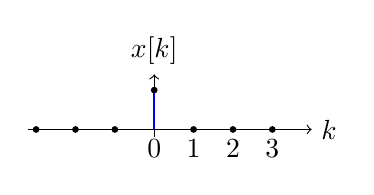
\begin{tikzpicture}[baseline=0.8,scale=0.5]
					      \draw[->] (0,-0.2) -- (0,1.4) node[above]{$x[k]$}; %y
					      \draw[->] (-3.2,0) -- (4,0) node[right]{$k$}; %x
					      \filldraw[black] (-3,0) circle (2pt) {};
					      \filldraw[black] (-2,0) circle (2pt) {};
					      \filldraw[black] (-1,0) circle (2pt) {};
					      \draw[blue, thick] (0,1) -- (0,0) node[below, black]{0}; \filldraw[black] (0,1) circle (2pt) {};
					      \filldraw[black] (1,0) circle (2pt) node[below]{1};
					      \filldraw[black] (2,0) circle (2pt) node[below]{2};
					      \filldraw[black] (3,0) circle (2pt) node[below]{3};
				      \end{tikzpicture}
			      \end{minipage}
		      }
		      Eigenschaften:
		      \begin{itemize}
			      \item neutrales Element der Faltung
			      \item Anregung der Impulsantwort
			      \item besitzt konstantes Spektrum
			      \item Summe ist $\sum^{\infty}_{n=-\infty}\delta(n)=1$
		      \end{itemize}
		      Ausblendeeigenschaft:
		      \[
			      x(n) = \sum_{k=-\infty}^{\infty} x(k)\cdot\delta(n-k)
		      \]
		\item \textbf{Einheitssprung}\\
		      \makebox[\textwidth][c]
		      {
			      \begin{minipage}{0.3\textwidth}
				      \[
					      \varepsilon(n) =
					      \begin{cases}
						      1 & n \geq 0 \\
						      0 & n < 0
					      \end{cases}
				      \]
			      \end{minipage}
			      \begin{minipage}{0.7\textwidth}
				      \centering
				      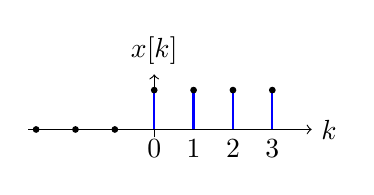
\begin{tikzpicture}[baseline=0.8,scale=0.5]
					      \draw[->] (0,-0.2) -- (0,1.4) node[above]{$x[k]$}; %y
					      \draw[->] (-3.2,0) -- (4,0) node[right]{$k$}; %x
					      \filldraw[black] (-3,0) circle (2pt) {};
					      \filldraw[black] (-2,0) circle (2pt) {};
					      \filldraw[black] (-1,0) circle (2pt) {};
					      \draw[blue, thick] (0,1) -- (0,0) node[below, black]{0}; \filldraw[black] (0,1) circle (2pt) {};
					      \draw[blue, thick] (1,1) -- (1,0) node[below, black]{1}; \filldraw[black] (1,1) circle (2pt) {};
					      \draw[blue, thick] (2,1) -- (2,0) node[below, black]{2}; \filldraw[black] (2,1) circle (2pt) {};
					      \draw[blue, thick] (3,1) -- (3,0) node[below, black]{3}; \filldraw[black] (3,1) circle (2pt) {};
				      \end{tikzpicture}
			      \end{minipage}
		      }
		      Zusammenhang mit Einheitsimpulse:
		      \[
			      \delta(n) = \varepsilon(n) - \varepsilon(n-1)
		      \]
		\item \textbf{Rechteckfolge}\\
		      \makebox[\textwidth][c]
		      {
			      \begin{minipage}{0.3\textwidth}
				      \[
					      \operatorname{rect}(n) =
					      \begin{cases}
						      1 & 0 \leq n < N   \\
						      0 & \texttt{sonst}
					      \end{cases}
				      \]
			      \end{minipage}
			      \begin{minipage}{0.7\textwidth}
				      \centering
				      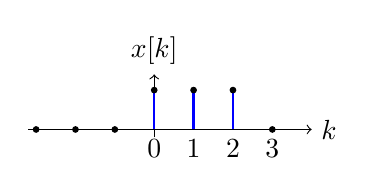
\begin{tikzpicture}[baseline=0.8,scale=0.5]
					      \draw[->] (0,-0.2) -- (0,1.4) node[above]{$x[k]$}; %y
					      \draw[->] (-3.2,0) -- (4,0) node[right]{$k$}; %x
					      \filldraw[black] (-3,0) circle (2pt) {};
					      \filldraw[black] (-2,0) circle (2pt) {};
					      \filldraw[black] (-1,0) circle (2pt) {};
					      \draw[blue, thick] (0,1) -- (0,0) node[below, black]{0}; \filldraw[black] (0,1) circle (2pt) {};
					      \draw[blue, thick] (1,1) -- (1,0) node[below, black]{1}; \filldraw[black] (1,1) circle (2pt) {};
					      \draw[blue, thick] (2,1) -- (2,0) node[below, black]{2}; \filldraw[black] (2,1) circle (2pt) {};
					      \filldraw[black] (3,0) circle (2pt) node[below] {3};
				      \end{tikzpicture}
			      \end{minipage}
		      }
		      Zusammenhang mit Dirac- und Einheitsimpuls:
		      \begin{align*}
			      \operatorname{rect}(n) & = \varepsilon(n) + \varepsilon(n-N)       \\
			                             & = \varepsilon(n) \cdot \varepsilon(N-1-n)
		      \end{align*}
		\item \textbf{Zeitdiskrete Sinus}\\
		      \makebox[\textwidth][c]
		      {
			      \begin{minipage}{0.3\textwidth}
				      \[
					      x(n) = A \cdot \sin(\Omega n+\varphi)
				      \]
			      \end{minipage}
			      \begin{minipage}{0.7\textwidth}
				      \centering
				      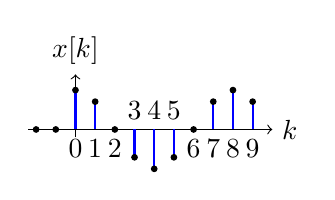
\begin{tikzpicture}[baseline=1,scale=0.5]
					      \draw[->] (0,-0.2) -- (0,1.4) node[above]{$x[k]$}; %y
					      \draw[->] (-1.2,0) -- (5,0) node[right]{$k$}; %x
					      \filldraw[black] (-1,0) circle (2pt) {};
					      \filldraw[black] (-0.5,0) circle (2pt) {};
					      \draw[blue,thick] (0,1) -- (0,0)          node[below, black]{0}; \filldraw[black] (0,1) circle (2pt) {};
					      \draw[blue,thick] (0.5,0.707) -- (0.5,0)  node[below, black]{1}; \filldraw[black] (0.5,0.707) circle (2pt) {};
					      \filldraw[black] (1,0) circle (2pt)              node[below, black]{2};
					      \draw[blue,thick] (1.5,-0.707) -- (1.5,0) node[above, black]{3}; \filldraw[black] (1.5,-0.707) circle (2pt) {};
					      \draw[blue,thick] (2,-1) -- (2,0)         node[above, black]{4}; \filldraw[black] (2,-1) circle (2pt) {};
					      \draw[blue,thick] (2.5,-0.707) -- (2.5,0) node[above, black]{5}; \filldraw[black] (2.5,-0.707) circle (2pt) {};
					      \filldraw[black] (3,0) circle (2pt)              node[below]{6};
					      \draw[blue,thick] (3.5,0.707) -- (3.5,0)  node[below, black]{7}; \filldraw[black] (3.5,0.707) circle (2pt) {};
					      \draw[blue,thick] (4,1) -- (4,0)          node[below, black]{8}; \filldraw[black] (4,1) circle (2pt) {};
					      \draw[blue,thick] (4.5,0.707) -- (4.5,0)  node[below, black]{9}; \filldraw[black] (4.5,0.707) circle (2pt) {};
				      \end{tikzpicture}
			      \end{minipage}
		      }
		      \footnotesize
		      \begin{align*}
			      A       & :\texttt{Amplitude}               \\
			      \Omega  & :\texttt{normierte Kreisfrequenz} \\
			      \varphi & :\texttt{Anfangsphase}
		      \end{align*}
		      \normalsize
		\item \textbf{Exponentialfolge}\\
		      \makebox[\textwidth][c]
		      {
			      \begin{minipage}{0.3\textwidth}
				      \begin{align*}
					      x(n) & = \underline{A} \cdot e^{Sn}                \\
					           & = \underline{A} \cdot e^{(\Sigma+j\Omega)n}
				      \end{align*}
			      \end{minipage}
			      \begin{minipage}{0.7\textwidth}
				      \centering
				      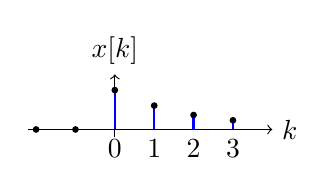
\begin{tikzpicture}[baseline=0.8,scale=0.5]
					      \draw[->] (0,-0.2) -- (0,1.4) node[above]{$x[k]$}; %y
					      \draw[->] (-2.2,0) -- (4,0) node[right]{$k$}; %x
					      \filldraw[black] (-2,0) circle (2pt) {};
					      \filldraw[black] (-1,0) circle (2pt) {};
					      \draw[blue, thick] (0,1) -- (0,0) node[below, black]{0}; \filldraw[black] (0,1) circle (2pt) {};
					      \draw[blue, thick] (1,0.606) -- (1,0) node[below, black]{1}; \filldraw[black] (1,0.606) circle (2pt) {};
					      \draw[blue, thick] (2,0.367) -- (2,0) node[below, black]{2}; \filldraw[black] (2,0.367) circle (2pt) {};
					      \draw[blue, thick] (3,0.233) -- (3,0) node[below, black]{3}; \filldraw[black] (3,0.233) circle (2pt) {};
				      \end{tikzpicture}
			      \end{minipage}
		      }
		      \begin{align*}
			      S &= \Sigma+j\Omega                                               \\
			       \texttt{Amplitudenänderung }\Sigma &= \sigma T = \sigma/f_A     \\
			       \texttt{normierte Kreisfrequenz }\Omega &= \omega T =  2\pi f_A
		      \end{align*}
	\end{itemize}
\end{mdframed}



\end{multicols*}
\end{document}
